\documentclass[a4paper,kul]{kulakarticle} %options: kul or kulak (default)

\usepackage[utf8]{inputenc}
\usepackage[english]{babel}
\usepackage{graphicx}
\usepackage{subcaption}
\newlength{\twosubht}
\newsavebox{\twosubbox}
\graphicspath{{../Figures/}{/}}
\usepackage[outdir=./]{epstopdf}

\usepackage{amsmath}
\usepackage{amsthm}
\usepackage{amssymb}
\usepackage{gensymb}
\setcounter{MaxMatrixCols}{21}

\usepackage{etoolbox,refcount}
\usepackage{multicol}

\newcounter{countitems}
\newcounter{nextitemizecount}
\newcommand{\setupcountitems}{%
	\stepcounter{nextitemizecount}%
	\setcounter{countitems}{0}%
	\preto\item{\stepcounter{countitems}}%
}
\makeatletter
\newcommand{\computecountitems}{%
	\edef\@currentlabel{\number\c@countitems}%
	\label{countitems@\number\numexpr\value{nextitemizecount}-1\relax}%
}
\newcommand{\nextitemizecount}{%
	\getrefnumber{countitems@\number\c@nextitemizecount}%
}
\newcommand{\previtemizecount}{%
	\getrefnumber{countitems@\number\numexpr\value{nextitemizecount}-1\relax}%
}
\makeatother    
\newenvironment{AutoMultiColItemize}{%
	\ifnumcomp{\nextitemizecount}{>}{3}{\begin{multicols}{2}}{}%
		\setupcountitems\begin{itemize}}%
		{\end{itemize}%
		\unskip\computecountitems\ifnumcomp{\previtemizecount}{>}{3}{\end{multicols}}{}}

\usepackage{pdflscape}

\date{Academic year 2021 -- 2022}
\address{
  Faculty of Engineering Science \\
  Department of Mechanical Engineering \\
  Control theory \texttt{[H04X3a]}}
\title{Report Assignment 1: identification of the motors}
\author{Toon Servaes, Matthias Derez}


\begin{document}

\maketitle

\section{Model Structure}
\subsection{Discrete-time Model Structure} 

In order to select the discrete-time model structure for the DC motors, the equivalent electric circuit in Figure \ref{fig:DCmotors} is used. By using Newton's second law and Kirchhoff's voltage law, following equations can be derived:

\begin{equation}
    \label{eq:circuit}
    \begin{split}
         J\ddot{\theta}  + b\dot{\theta} &= K_{t}i \\
         L\frac{di}{dt} + Ri &= V - K_{e}\dot{\theta}
     \end{split} 
\end{equation}
The meaning of each parameter is:
\begin{itemize}
    \item $J$ = moment of inertia of the rotor [kg $\cdot$ m$^2$]
    \item $\theta$ = angular position [rad]
    \item $b$ = motor viscous friction constant [N $\cdot$ m $\cdot$ s]
    \item $K_{e}$ = electromotive force constant [$\frac{\text{V}}{\text{rad } \cdot \text{ s}}$] = $K_{t}$ = motor torque constant [$\frac{\text{N } \cdot \text{ m}}{\text{A }}$] = $K$
    \item $R$ = electric resistance [$\ohm$]
    \item $L$ = electric inductance [H]
\end{itemize}

\subsubsection*{Continuous-time Transfer Function}
Applying the Laplace transform to both equations in (\ref{eq:circuit}) leads to:

\begin{equation}
\begin{split}
	&Js^2\Theta(s) + bs\Theta(s) = KI(s) \\
	&LsI(s) + RI(s) = V(s) - Ks\Theta(s)	
\end{split}
\end{equation}
assuming $\theta(0) = 0$, $\dot{\theta}(0) = 0 \text{ and } i(0) = 0$. After some calculations, the continuous-time transfer function describing the behaviour of this system can be derived:
\begin{equation}
	\label{eq:TF}
    H(s) = \frac{\dot{\Theta}(s)}{V(s)} = \frac{s\Theta(s)}{V(s)} = \frac{K}{(Js + b)(Ls + R) + K^2}
\end{equation}
where the input is the voltage source $V(s)$ applied to the motor's armature and the output is the rotational velocity of the wheel  $\dot{\Theta}(s)$. One can rewrite this transfer function in order to obtain a more general and well-known form:
\begin{equation}
\label{eq:TF2}
\begin{split}
	H(s) &= \frac{K}{(Js + b)(Ls + R) + K^2} \\
	 &= \frac{K}{LJs^2 + (Lb + JR)s + K^2 + bR} \\
	 &= \frac{\frac{K}{LJ}}{s^2 + \frac{Lb + JR}{LJ}s + \frac{K^2 + bR}{LJ}} \\
	 &= C \frac{\omega_n^2}{s^2 + 2\zeta\omega_ns + \omega_n^2}
\end{split}
\end{equation}
where $C = \frac{K}{K^2 + bR}$, $\omega_n^2 = \frac{K^2 + bR}{LJ}$ and $\zeta = \frac{Lb+JR}{2\sqrt{LJ(K^2 + bR)}}$.


\begin{figure}[htp!]
    \centering
    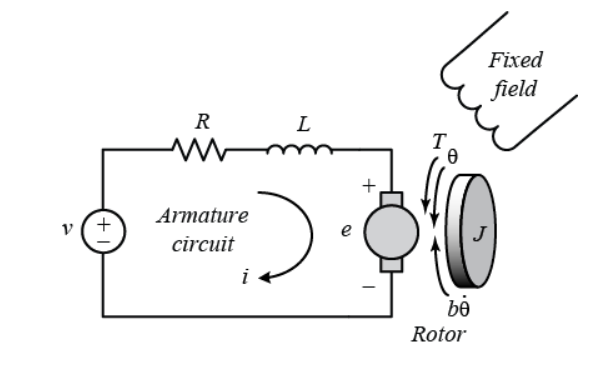
\includegraphics[width=.6\linewidth]{DC_motors.png}
    \caption{Electric equivalent circuit of the armature and the free-body diagram of the rotor.}
    \label{fig:DCmotors}
\end{figure}


\subsubsection*{Discrete-time Transfer Function}

The discrete-time transfer function is derived from the continuous-time one by using a zero-order hold sampling process. To this extent, one has to compute $H(z) = (1-z^{-1}) \mathcal{Z} (\mathcal{L}^{-1}\{\frac{H(s)}{s}\} \times \delta_T(t))$. The software running on the Arduino, called 'MicroOS', samples at $100$ Hz. Consequently, the sampling period $T_s = 0.01$ s. 
\\\\
Firstly, Equation (\ref{eq:TF2}) can be rewritten as follows: 
\begin{equation}
	H(s) = C \frac{\omega_n^2}{s^2 + 2\zeta\omega_ns + \omega_n^2} = C \frac{a^2 + b^2}{(s+a)^2 + b^2}
\end{equation}
where $a = \zeta\omega_n$ and $b = \sqrt{\omega_n^2(1-\zeta^2)}$. Next, using transform pair no. 22 on page 4 of the course formulary leads to:
\begin{equation}
	\mathcal{Z} \left(\mathcal{L}^{-1}\left\{\frac{H(s)}{s}\right\} \times \delta_T(t)\right) = \frac{z(Az+B)}{(z-1)\left[z^2-2e^{-aT_s}\cos(bT_s)z+e^{-2aT_s}\right]}
\end{equation}
where $A = 1-e^{-aT_s}\cos(bT_s) - \frac{a}{b}e^{-aT_s}\sin(bT_s)$ and $B = e^{-2aT_s}\cos(bT_s) + \frac{a}{b}e^{-aT_s}\sin(bT_s) - e^{-aT_s}\cos(bT_s)$. Finally, the zero-order hold equivalent is determined:
\begin{equation}
	H(z) = (1-z^{-1})\mathcal{Z} \left(\mathcal{L}^{-1}\left\{\frac{H(s)}{s}\right\} \times \delta_T(t)\right) = \frac{(Az+B)}{\left[z^2-2e^{-aT_s}\cos(bT_s)z+e^{-2aT_s}\right]}
\end{equation}
More generally: 
\begin{equation}
	H(z) = \frac{b_0z + b_1}{z^2 + a_0 z + a_1}
\end{equation}
However, the MicroOS software on the Arduino stores the control command calculated during discrete-time interval $k$ in a memory buffer until discrete-time instance $k+1$. In this way, the delay between the measurement of the output and sending out of the control command is increased by one sampling period $T_s$. In the $z$-domain, this is equivalent to a multiplication of the transfer function by $z^{-1}$, leading to the final, generalised discrete-time transfer function of the system:
\begin{equation}
	H(z) = \frac{b_0z + b_1}{z^3 + a_0 z^2 + a_1 z}
\end{equation}
The order of the numerator is 1, while the order of the denominator is 3. This is in line with the strict causality condition, which demands that the order of the numerator is strictly smaller than the denominator. 
\\\\
This is the transfer function that is used in the rest of the assignment. The unknown parameters $b_0$, $b_1$, $a_0$ and $a_1$ are determined in Section X using the least-squares method. This is done for each motor separately.

\subsection{Input and Output}
As previously mentioned, the input of the model is the voltage source $V(s)$ applied to the motor's armature. This voltage is controlled by the Arduino and is expressed in Volts [V]. The output is the rotational velocity of the wheel  $\dot{\Theta}(s)$, expressed in [rad/s].

% ---------------------------------------------------------------------------

\section{Identification of each 'DC Motor + Wheel'}
\subsection{Excitation Signal}
In order to identify the system 'DC motor + wheel', it is necessary to perform a dedicated experiment that actively excites the system, while the \textit{persistency of excitation} condition is satisfied. This means that the excitation should be suf


\subsection{System Parameters}

\subsection{Filtering}






\begin{figure}[htp!]
    \centering
    \includegraphics[width=.7\linewidth]{input_voltage.eps}
    \caption{Input voltage}
    \label{fig:input_voltage}
\end{figure}

\begin{figure}[htp!]
    \centering
    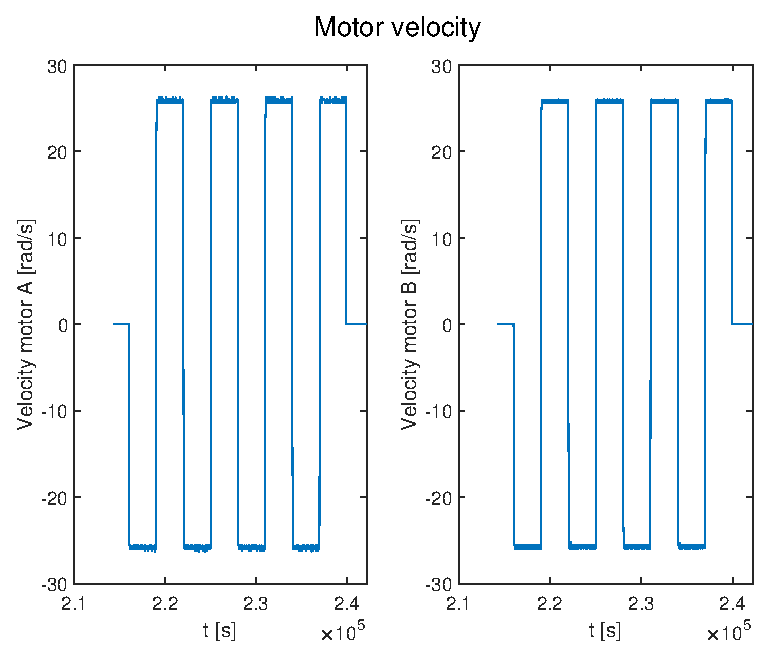
\includegraphics[width=.7\linewidth]{motor_velocity.eps}
    \caption{Motor velocity}
    \label{fig:motor_velocity}
\end{figure}



\section*{Conclusion}
Yeet
\end{document}